% ======================= CHƯƠNG 4: THÍ NGHIỆM VÀ KẾT QUẢ ==========================
\chapter{Thí nghiệm và Kết quả}

Mọi thí nghiệm chạy trên GPU 4~GB duy nhất mô tả ở Mục~3.3, với hạt giống ngẫu nhiên cố định bằng 42. Kết quả được báo cáo trên tập kiểm tra giữ riêng gồm hai mươi video (mã 61--80), tập mà không mô hình nào thấy trong lúc huấn luyện hay chọn mô hình.

\section{So sánh Ba Mô hình}

\subsection{Kết quả Tổng thể}

Bảng~\ref{tab:vn_model_comparison} báo cáo độ chính xác và Macro-F1 cho ba mô hình, trước và sau khi làm mượt trung vị.

\begin{table}[H]
\centering
\caption{Kết quả trên tập kiểm tra cho ba mô hình. Giá trị tốt nhất in \textbf{đậm}.}
\label{tab:vn_model_comparison}
\begin{tabular}{lcccc}
\toprule
\textbf{Mô hình} & \textbf{Acc. thô} & \textbf{Macro-F1 thô} & \textbf{Acc. mượt} & \textbf{Macro-F1 mượt} \\
\midrule
M1 --- ResNet-50 + BiLSTM      & 0,832 & 0,775 & 0,837 & 0,781 \\
M2 --- EfficientNet-B3 + TCN   & 0,818 & 0,739 & 0,824 & 0,748 \\
\textbf{M3 --- Swin-Tiny + Transformer} & \textbf{0,857} & \textbf{0,807} & \textbf{0,862} & \textbf{0,815} \\
\bottomrule
\end{tabular}
\end{table}

Swin-Transformer M3 tốt nhất trên mọi chỉ số, với Macro-F1 đã làm mượt là \textbf{0,815} --- cao hơn ResNet-LSTM 3,4 điểm và cao hơn EfficientNet-TCN 6,7 điểm. Độ chính xác 0,862 của nó nằm cùng khoảng với Trans-SVNet trên tập dữ liệu này, dù chỉ được huấn luyện trên một GPU laptop 4~GB. Hình~\ref{fig:vn_arch_compare} vẽ điểm số của mỗi mô hình theo số tham số: M3 thắng dù không phải mô hình lớn nhất, và M1 có nhiều tham số hơn nhưng điểm lại thấp hơn, nên kích thước mô hình không phải là yếu tố giới hạn kết quả ở đây.

\begin{figure}[H]
\centering
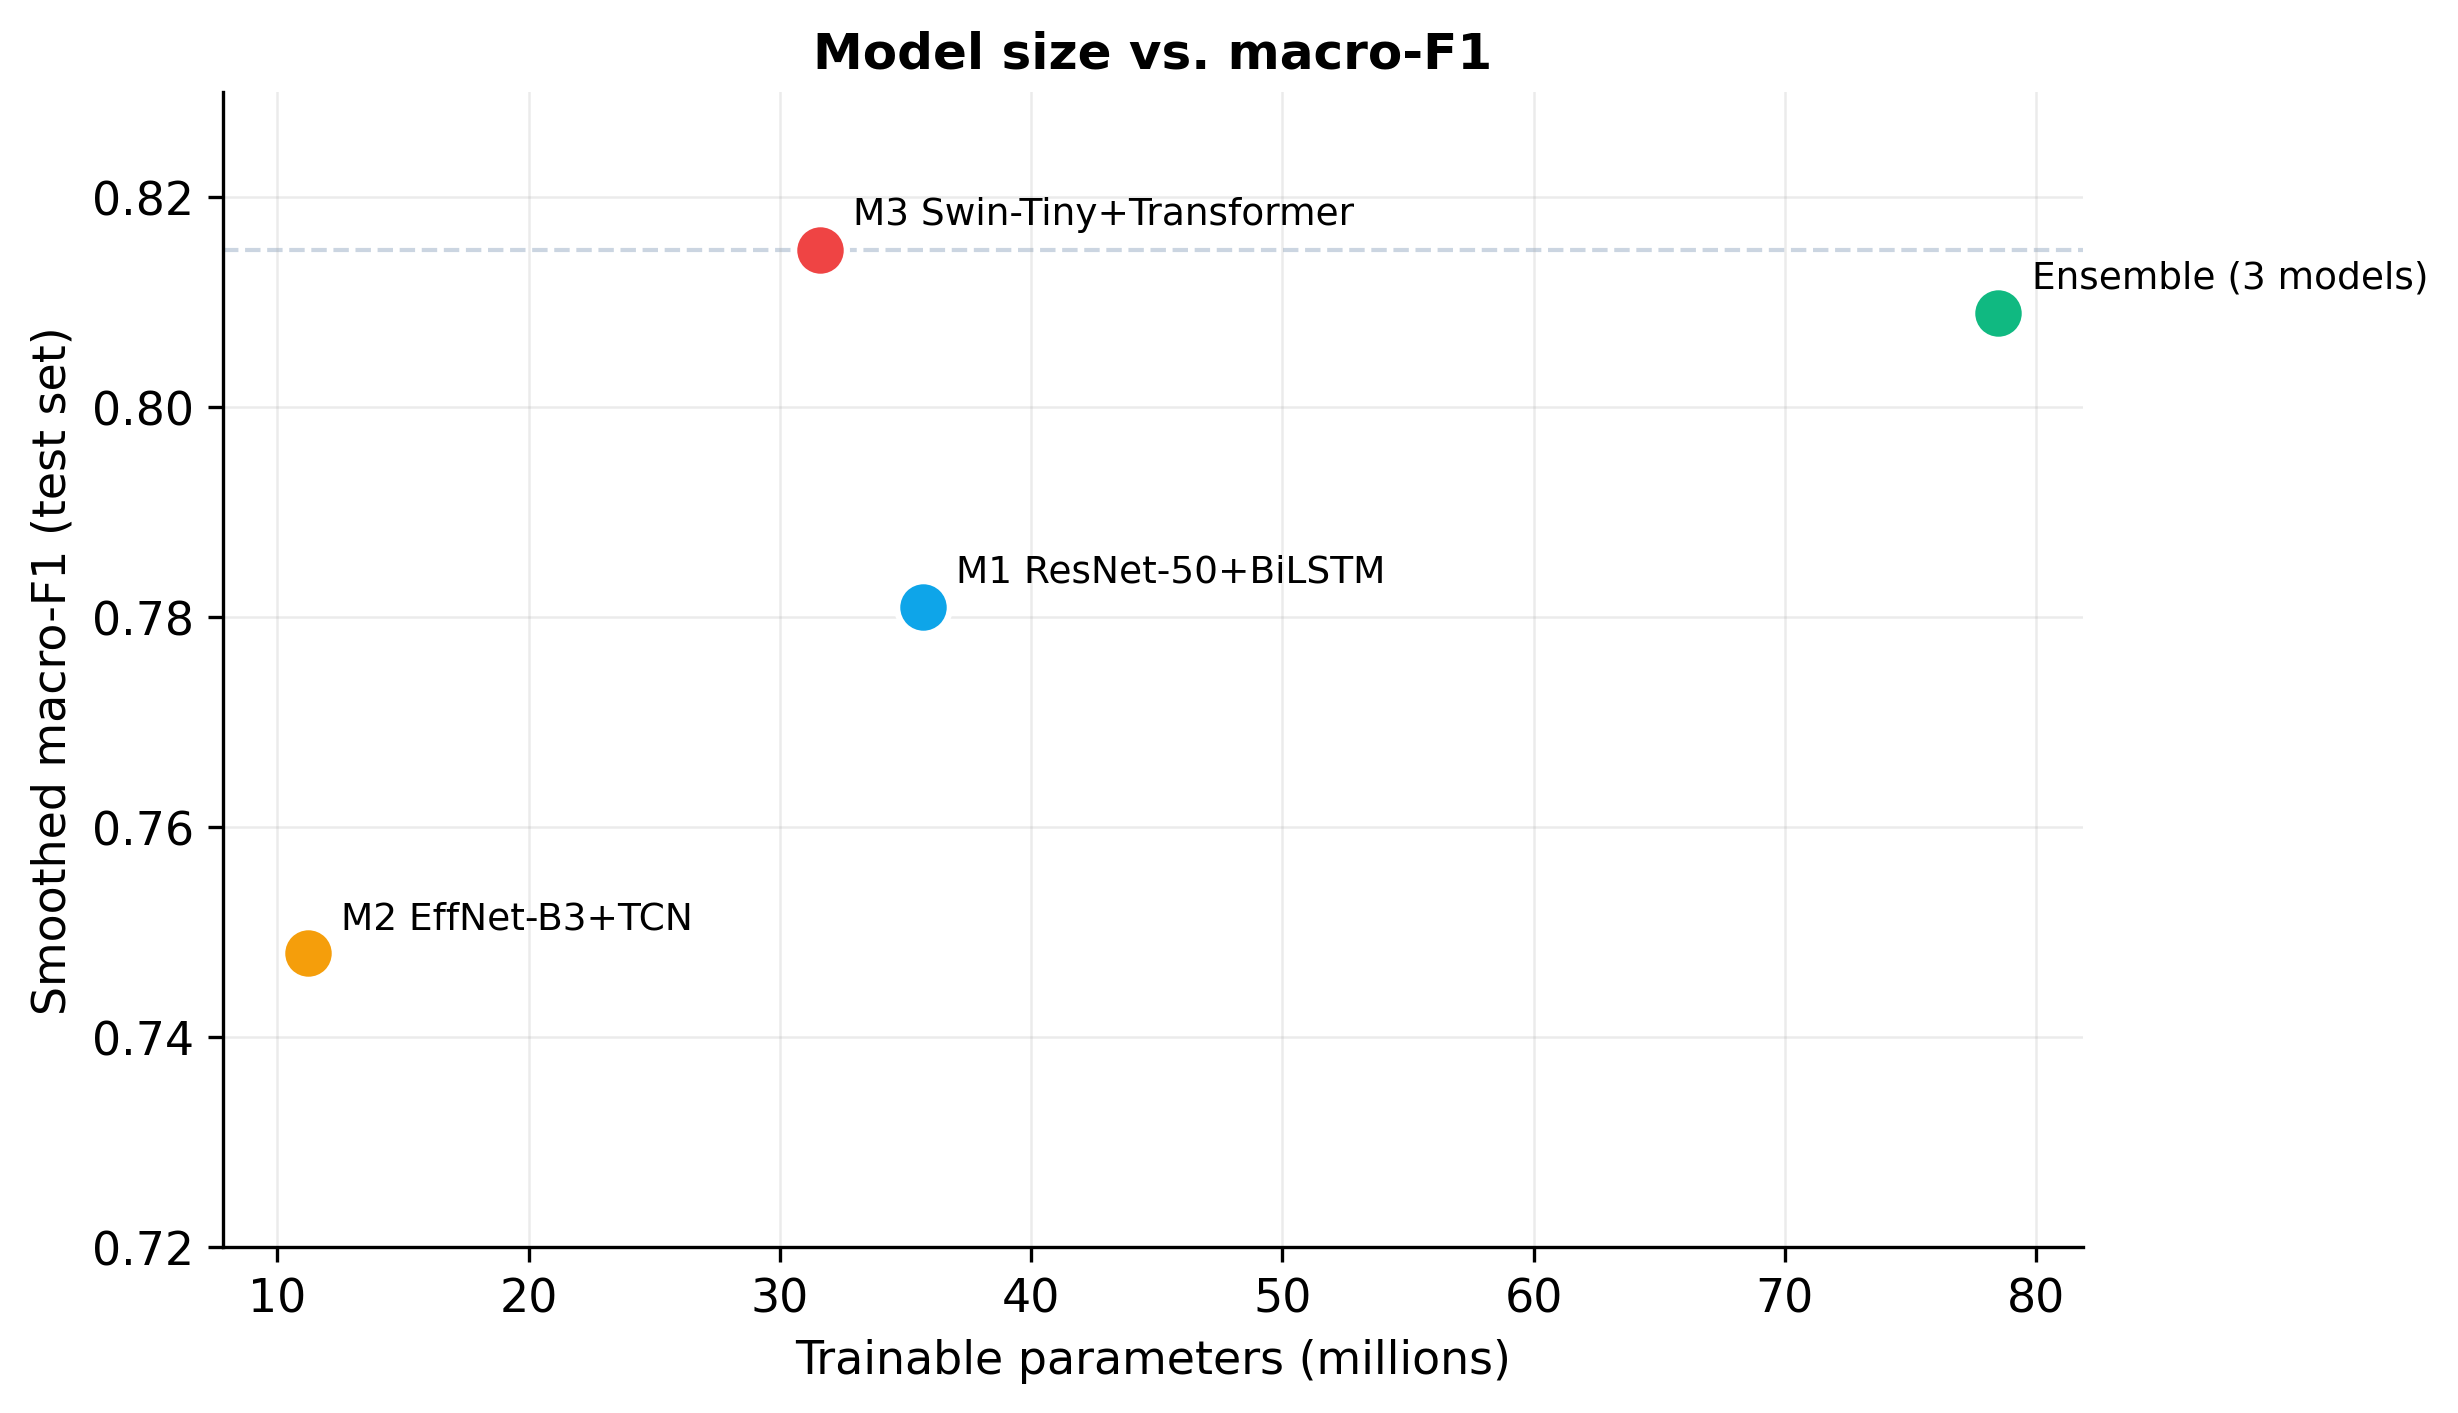
\includegraphics[width=\figwidth]{figures/arch_compare.png}
\caption{Kích thước mô hình so với Macro-F1. Swin-Transformer (M3) đạt điểm cao nhất dù không phải mô hình lớn nhất; EfficientNet-TCN (M2) nhỏ nhất và yếu nhất, một phần vì giai đoạn tinh chỉnh thứ ba của nó bị cắt ngắn do bộ nhớ hạn chế.}
\label{fig:vn_arch_compare}
\end{figure}

\subsection{Diễn biến Huấn luyện}

Hình~\ref{fig:vn_training_history} cho thấy đường cong mất mát và độ chính xác của ba mô hình qua ba giai đoạn. M1 và M3 huấn luyện trơn tru, và độ chính xác kiểm định của chúng tăng vọt ngay khi mạng nền được mở băng ở Giai đoạn 3. Đường của M2 ngắn hơn: với mạng nền EfficientNet-B3 được mở băng, mức dùng bộ nhớ đạt khoảng 97\% giới hạn 4~GB và chỉ một phần Giai đoạn 3 hoàn tất, nên các con số của M2 là cận dưới so với mức nó có thể đạt được nếu có nhiều bộ nhớ hơn.

\begin{figure}[H]
\centering
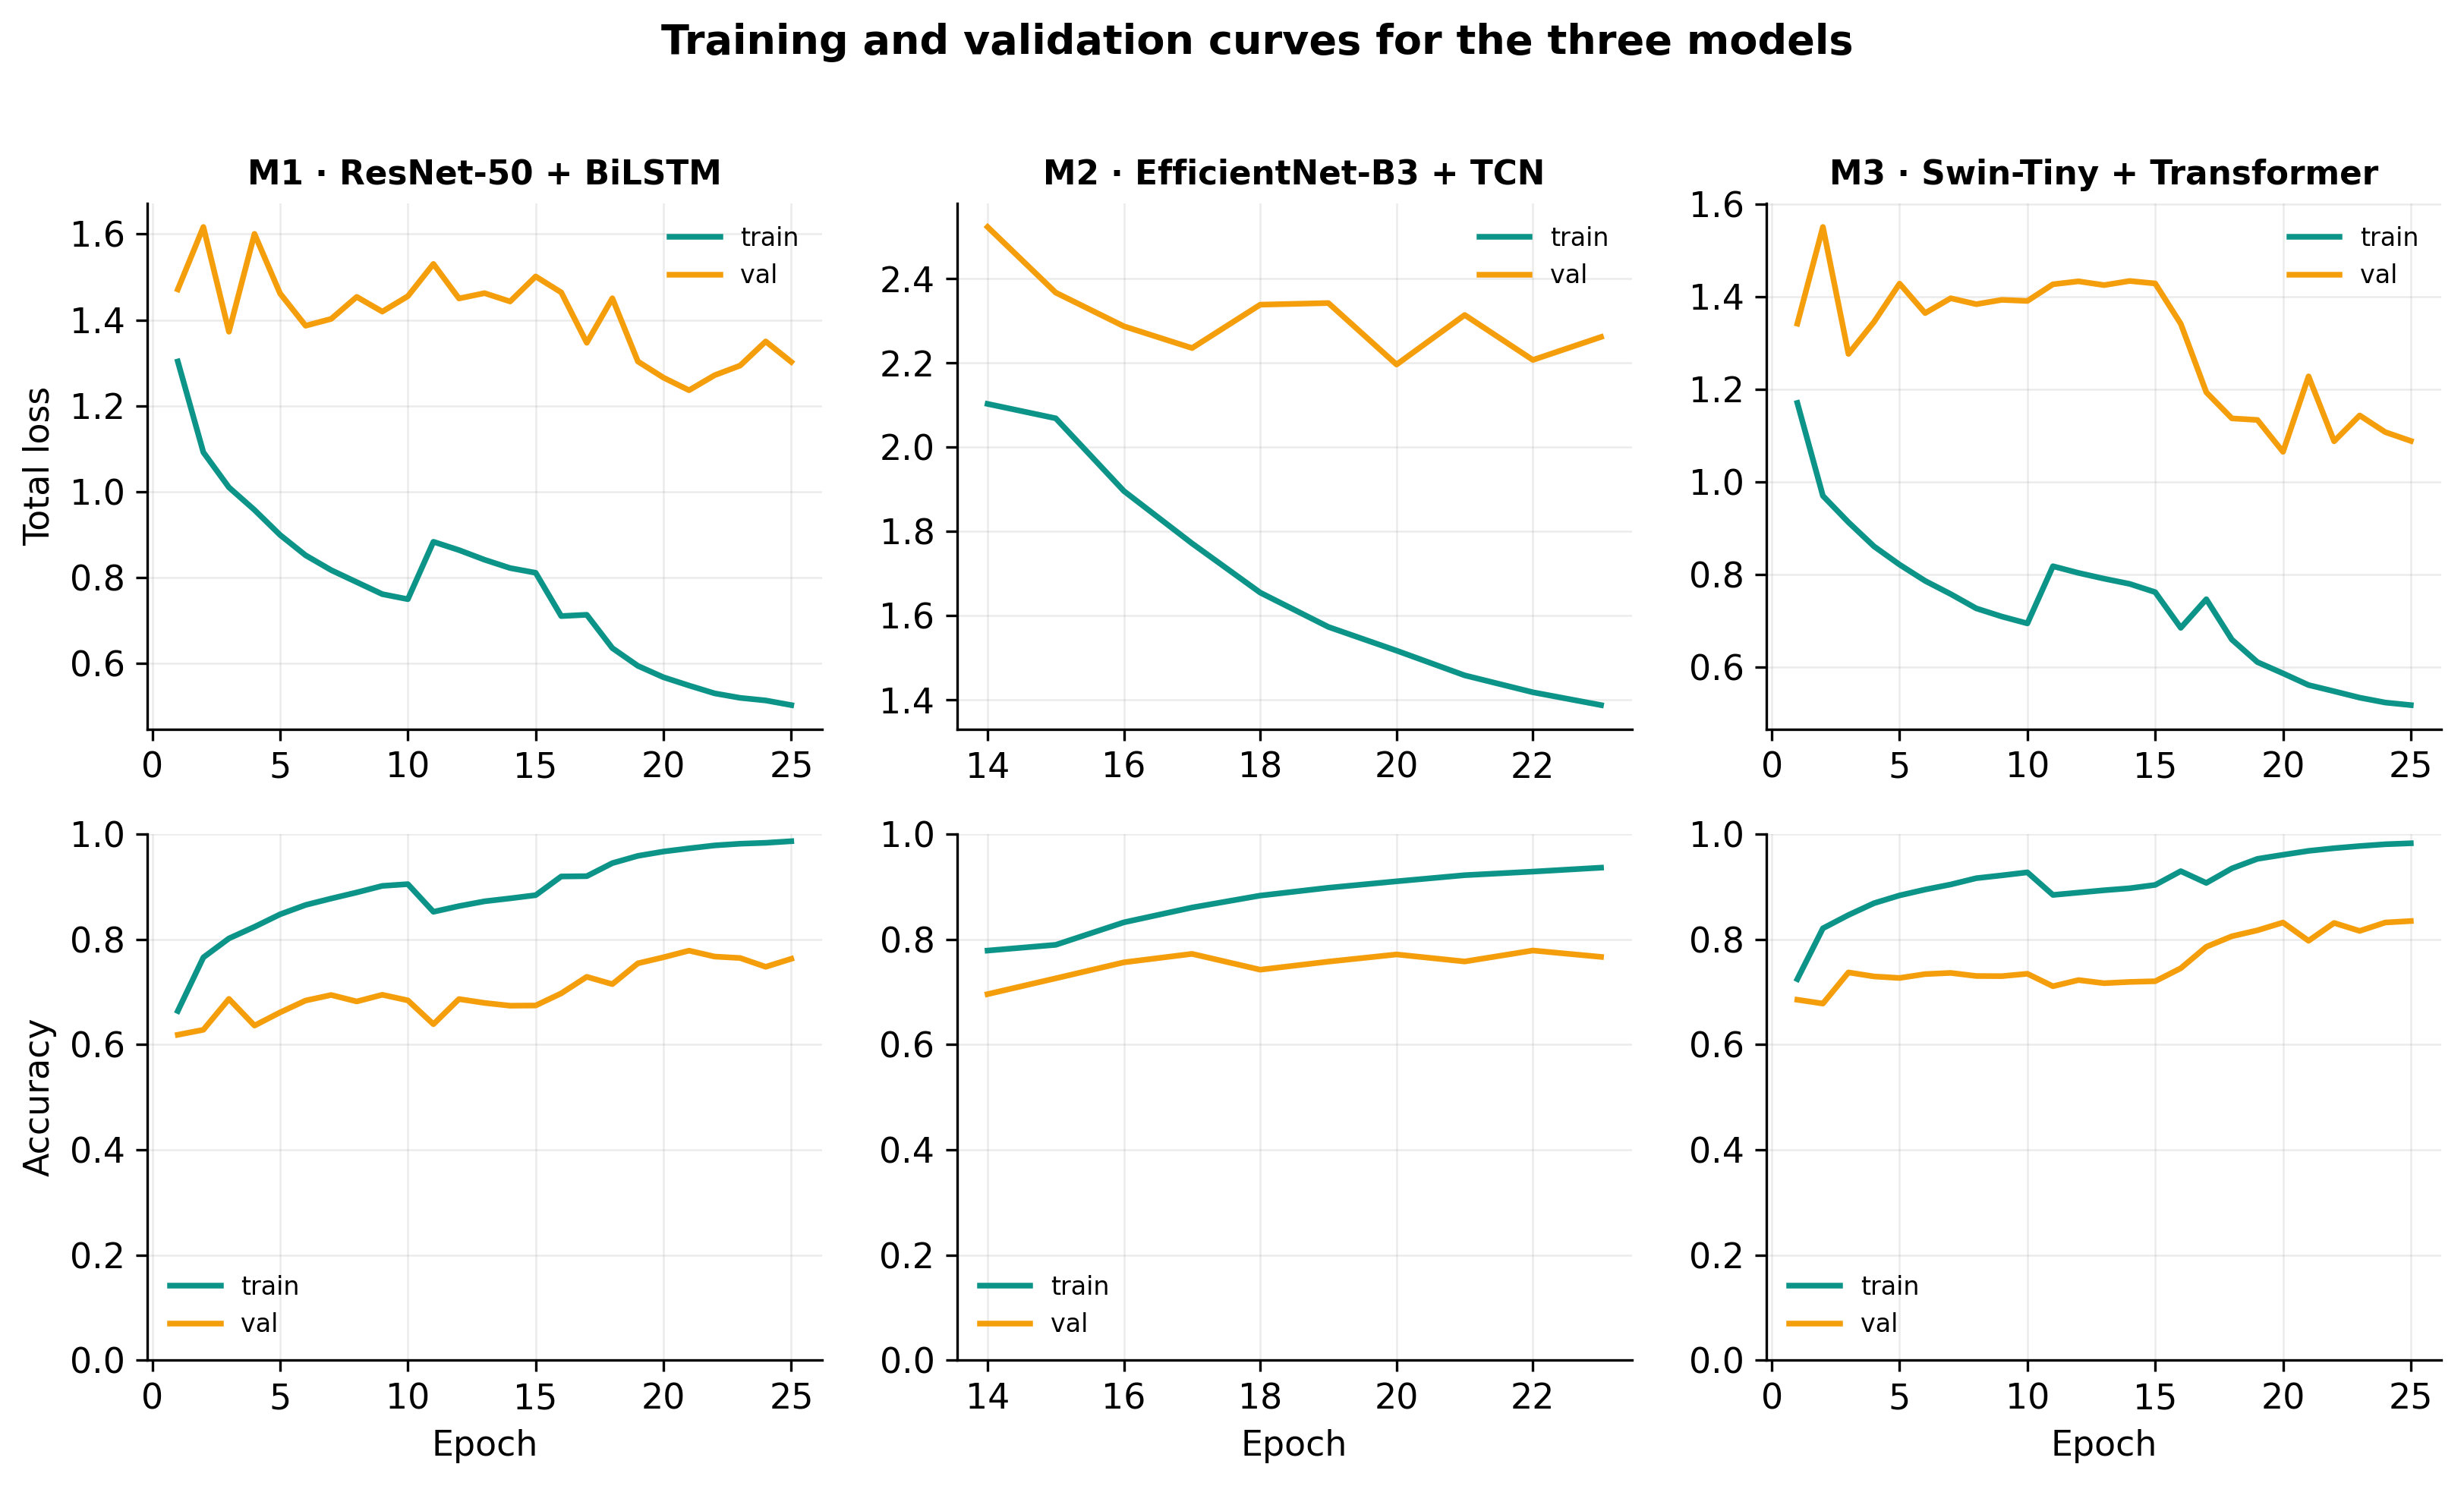
\includegraphics[width=\textwidth]{figures/train_history.png}
\caption{Mất mát và độ chính xác huấn luyện cùng kiểm định qua các epoch cho ba mô hình. M3 cho bước nhảy rõ nhất ở Giai đoạn 3; lần chạy của M2 bị cắt ngắn do bộ nhớ hạn chế khi tinh chỉnh mạng nền.}
\label{fig:vn_training_history}
\end{figure}

\subsection{Phân tích Theo từng Pha}

Bảng~\ref{tab:vn_per_class_m3} trình bày chi tiết precision, recall và F1 theo từng pha cho M3 trên các dự đoán thô của tập kiểm tra.

\begin{table}[H]
\centering
\caption{Precision, recall và F1 theo từng pha cho M3 (dự đoán thô, tập kiểm tra). Pha yếu nhất in \textbf{đậm}.}
\label{tab:vn_per_class_m3}
\begin{tabular}{lccc}
\toprule
\textbf{Pha} & \textbf{Precision} & \textbf{Recall} & \textbf{F1} \\
\midrule
Chuẩn bị                 & 0,830 & 0,803 & 0,816 \\
Bóc tách tam giác Calot  & 0,880 & 0,895 & 0,887 \\
Kẹp và cắt               & 0,815 & 0,796 & 0,806 \\
Bóc tách túi mật         & 0,868 & 0,885 & 0,877 \\
Đóng gói túi mật         & 0,881 & 0,759 & 0,816 \\
Làm sạch và đông máu     & 0,741 & 0,663 & \textbf{0,700} \\
Lấy túi mật ra           & 0,727 & 0,764 & 0,745 \\
\bottomrule
\end{tabular}
\end{table}

Hai pha phổ biến có F1 cao nhất, đúng như mong đợi. Pha yếu nhất là Làm sạch và đông máu (recall 0,663): mô hình thường nhầm việc làm sạch với pha bóc tách xung quanh, điều cũng thấy rõ trong ma trận nhầm lẫn (Hình~\ref{fig:vn_confusion_m3}). Quan trọng là cả bảy pha đều trên F1 $=0{,}70$, nên hàm mất mát có trọng số lớp thực sự ngăn được mô hình sụp về các pha phổ biến.

\begin{figure}[H]
\centering
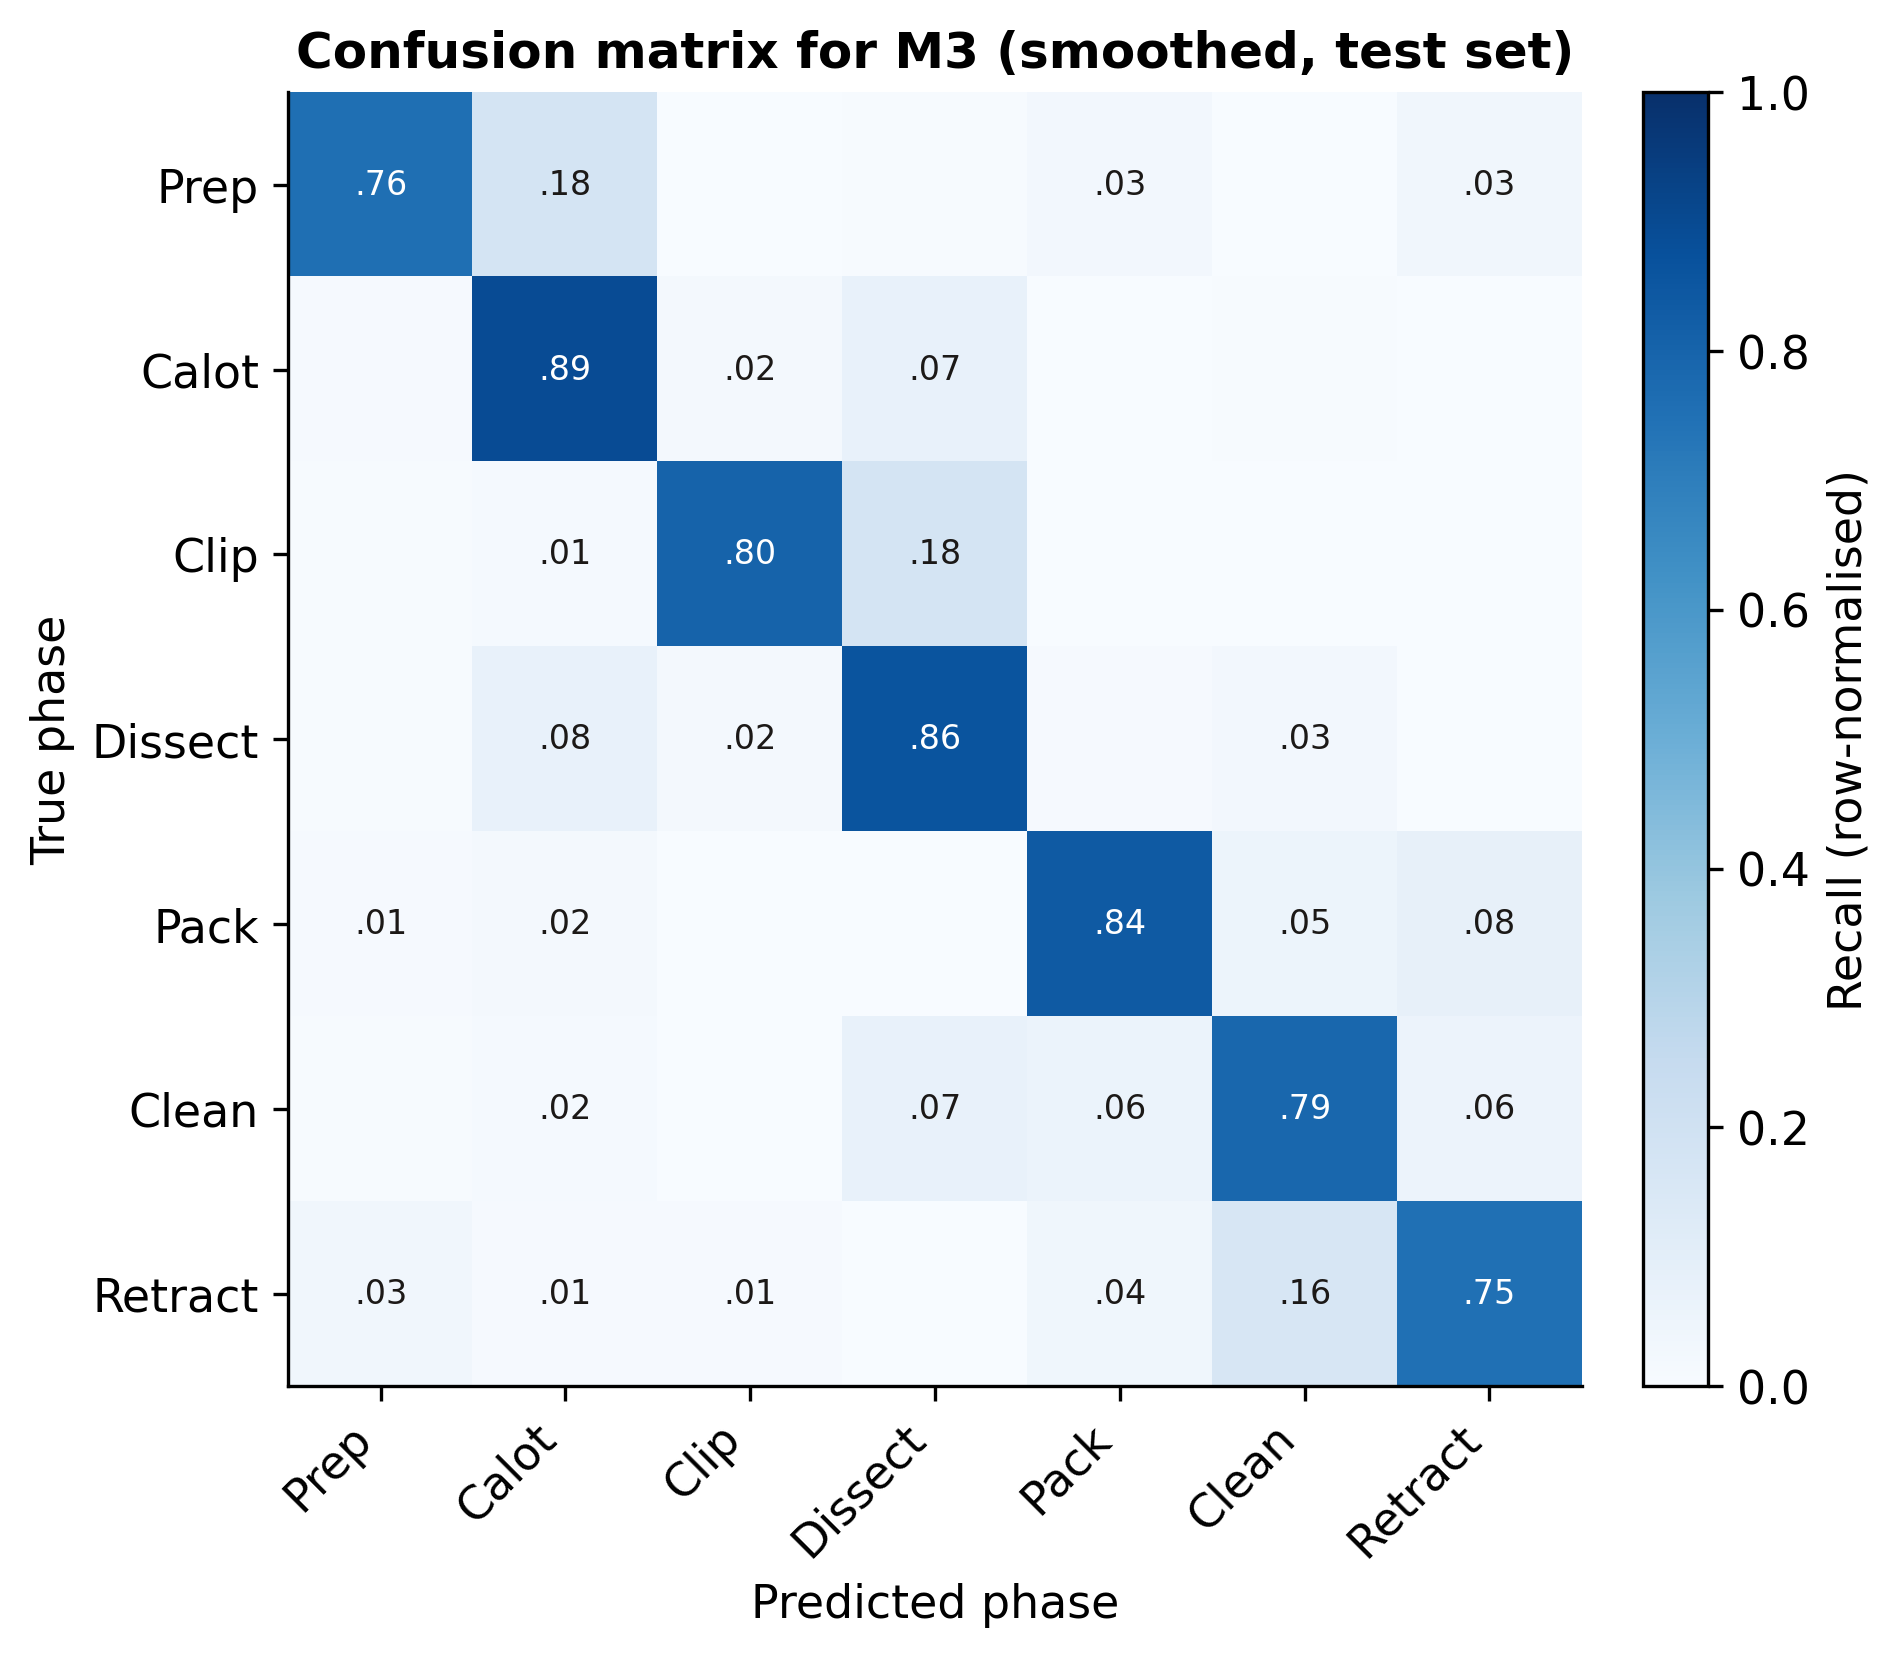
\includegraphics[width=\figwidth]{figures/confusion_m3.png}
\caption{Ma trận nhầm lẫn (mỗi hàng cộng lại bằng 1) cho M3 trên các dự đoán đã làm mượt của tập kiểm tra. Lỗi chính là Làm sạch và Kẹp bị dự đoán thành Bóc tách --- các pha lân cận trông giống nhau --- và không pha nào sụp về các pha phổ biến.}
\label{fig:vn_confusion_m3}
\end{figure}

\section{Nghiên cứu Loại bỏ}
\label{sec:vn_ablation}

Bảng~\ref{tab:vn_ablation} báo cáo bốn nghiên cứu loại bỏ so với mô hình cơ sở M1, tất cả đều huấn luyện với cùng bộ tối ưu và lịch trình ba giai đoạn.

\begin{table}[H]
\centering
\caption{Nghiên cứu loại bỏ (Macro-F1 đã làm mượt trên tập kiểm tra, thay đổi so với M1).}
\label{tab:vn_ablation}
\begin{tabular}{llcc}
\toprule
\textbf{Mã} & \textbf{Thay đổi} & \textbf{Macro-F1 mượt} & \textbf{$\Delta$F1 so với M1}\\
\midrule
\textbf{M1 cơ sở} & cấu hình đầy đủ & \textbf{0,781} & --- \\
\midrule
A1 & bỏ phát hiện dụng cụ (chỉ một nhiệm vụ) & 0,765 & $-1{,}6\%$ \\
A2 & bỏ đánh trọng số lớp                   & 0,761 & $-2{,}0\%$ \\
A3 & chuỗi 16 thay vì 8                     & 0,787 & $+0{,}6\%$ \\
A4 & tắt làm mượt trung vị                  & 0,775 & $-0{,}6\%$ \\
\bottomrule
\end{tabular}
\end{table}

Ba điểm nổi bật. Thứ nhất, bỏ nhiệm vụ dụng cụ (A1) làm mất 1,6 điểm Macro-F1, xác nhận rằng nhiệm vụ phụ này có ích, như EndoNet đã lưu ý đầu tiên. Thứ hai, bỏ đánh trọng số lớp (A2) làm mất 2,0 điểm, nhưng tổn thất không đều: hai pha hiếm nhất --- Lấy túi mật ra và Đóng gói --- mất 5,1 và 2,8 điểm F1 theo pha, trong khi pha phổ biến Calot lại tăng 0,7. Đây đúng là vấn đề mà đánh trọng số lớp được dùng để khắc phục. Thứ ba, A4 cho thấy bộ lọc trung vị làm gì: nó gần như không đổi Macro-F1 ($+0{,}6\%$) nhưng cải thiện điểm edit khoảng 35\%, nên vai trò chính của nó là làm sạch chuỗi pha chứ không phải cải thiện độ chính xác từng khung hình. Tăng gấp đôi độ dài chuỗi (A3) chỉ cho $+0{,}6\%$, nghĩa là cửa sổ tám giây đã bao phủ phần lớn ngữ cảnh hữu ích.

Cộng lại, đánh trọng số lớp và nhiệm vụ dụng cụ đáng giá gần bốn điểm Macro-F1 --- gần bằng khoảng cách 3,4 điểm giữa kiến trúc tốt nhất và kém nhất. Đây là bằng chứng chính cho thấy, trên Cholec80, công thức huấn luyện quan trọng ngang với mạng nền.

\section{Kết quả Kết hợp Mô hình}

Bảng~\ref{tab:vn_ensemble} so sánh ba cách kết hợp các mô hình.

\begin{table}[H]
\centering
\caption{Kết hợp ba mô hình (đã làm mượt, tập kiểm tra). Giá trị tốt nhất in \textbf{đậm}.}
\label{tab:vn_ensemble}
\begin{tabular}{lcc}
\toprule
\textbf{Chiến lược} & \textbf{Độ chính xác} & \textbf{Macro-F1} \\
\midrule
M3 đơn lẻ (mô hình đơn tốt nhất)        & 0,856 & 0,799 \\
Kết hợp --- trung bình softmax đơn giản & 0,863 & 0,808 \\
\textbf{Kết hợp --- trung bình theo F1 kiểm định} & \textbf{0,864} & \textbf{0,809} \\
Kết hợp --- biểu quyết đa số            & 0,857 & 0,799 \\
\bottomrule
\end{tabular}
\end{table}

Trung bình có trọng số theo F1 vượt mô hình đơn tốt nhất 1,0 điểm Macro-F1, với M3 nhận trọng số lớn nhất (0,355), rồi M1 (0,327) và M2 (0,318). Các trọng số gần như bằng nhau, gợi ý rằng ba mô hình đều có năng lực nhưng mắc lỗi tương tự nhau --- chúng có xu hướng sai trên cùng những khung hình khó (thường gần điểm chuyển pha) chứ không phải trên những khung hình khác nhau. Đây là lý do mục tiếp theo chuyển sang giải mã và hiệu chuẩn: nếu các lỗi còn lại tập trung và có cấu trúc, thì một bộ giải mã tốt hơn có thể giúp ích nhiều hơn là thêm mô hình.

\section{Giải mã Thời gian thực và Hiệu chuẩn}
\label{sec:vn_calibration}

Mục này so sánh bộ giải mã thời gian thực ở Mục~\ref{sec:vn_decoding} với các phương pháp đối chứng, dùng cùng các điểm số theo từng khung hình cho mọi phương pháp sao cho mọi khác biệt chỉ đến từ bước giải mã.

\subsection{Hiệu chuẩn}

Bảng~\ref{tab:vn_calibration} báo cáo ECE và NLL trên tập kiểm định trước và sau co giãn nhiệt độ. M1, mô hình quá tự tin nhất, được lợi nhiều nhất --- ECE của nó giảm 66\%. Với cả ba mô hình, nhiệt độ tốt nhất đều lớn hơn 1,0, dấu hiệu của sự quá tự tin. Hình~\ref{fig:vn_reliability} cho thấy các biểu đồ độ tin cậy: độ chính xác thô nằm dưới đường chéo ở các khoảng tin cậy cao, và co giãn nhiệt độ kéo đường cong trở lại về phía đường chéo.

\begin{table}[H]
\centering
\caption{Hiệu chuẩn trên tập kiểm định trước và sau co giãn nhiệt độ. ECE tốt nhất in \textbf{đậm}.}
\label{tab:vn_calibration}
\begin{tabular}{lccccc}
\toprule
\textbf{Mô hình} & \textbf{$T^\star$} & \textbf{ECE thô} & \textbf{ECE hc} & \textbf{NLL thô} & \textbf{NLL hc} \\
\midrule
M1 --- ResNet-LSTM      & 1,30 & 0,109 & \textbf{0,037} & 0,897 & 0,855 \\
M2 --- EffNet-TCN       & 1,10 & 0,059 & 0,074 & 0,824 & 0,817 \\
M3 --- Swin-Transformer & 1,20 & 0,074 & 0,070 & 0,688 & 0,667 \\
\bottomrule
\end{tabular}
\end{table}

\begin{figure}[H]
\centering
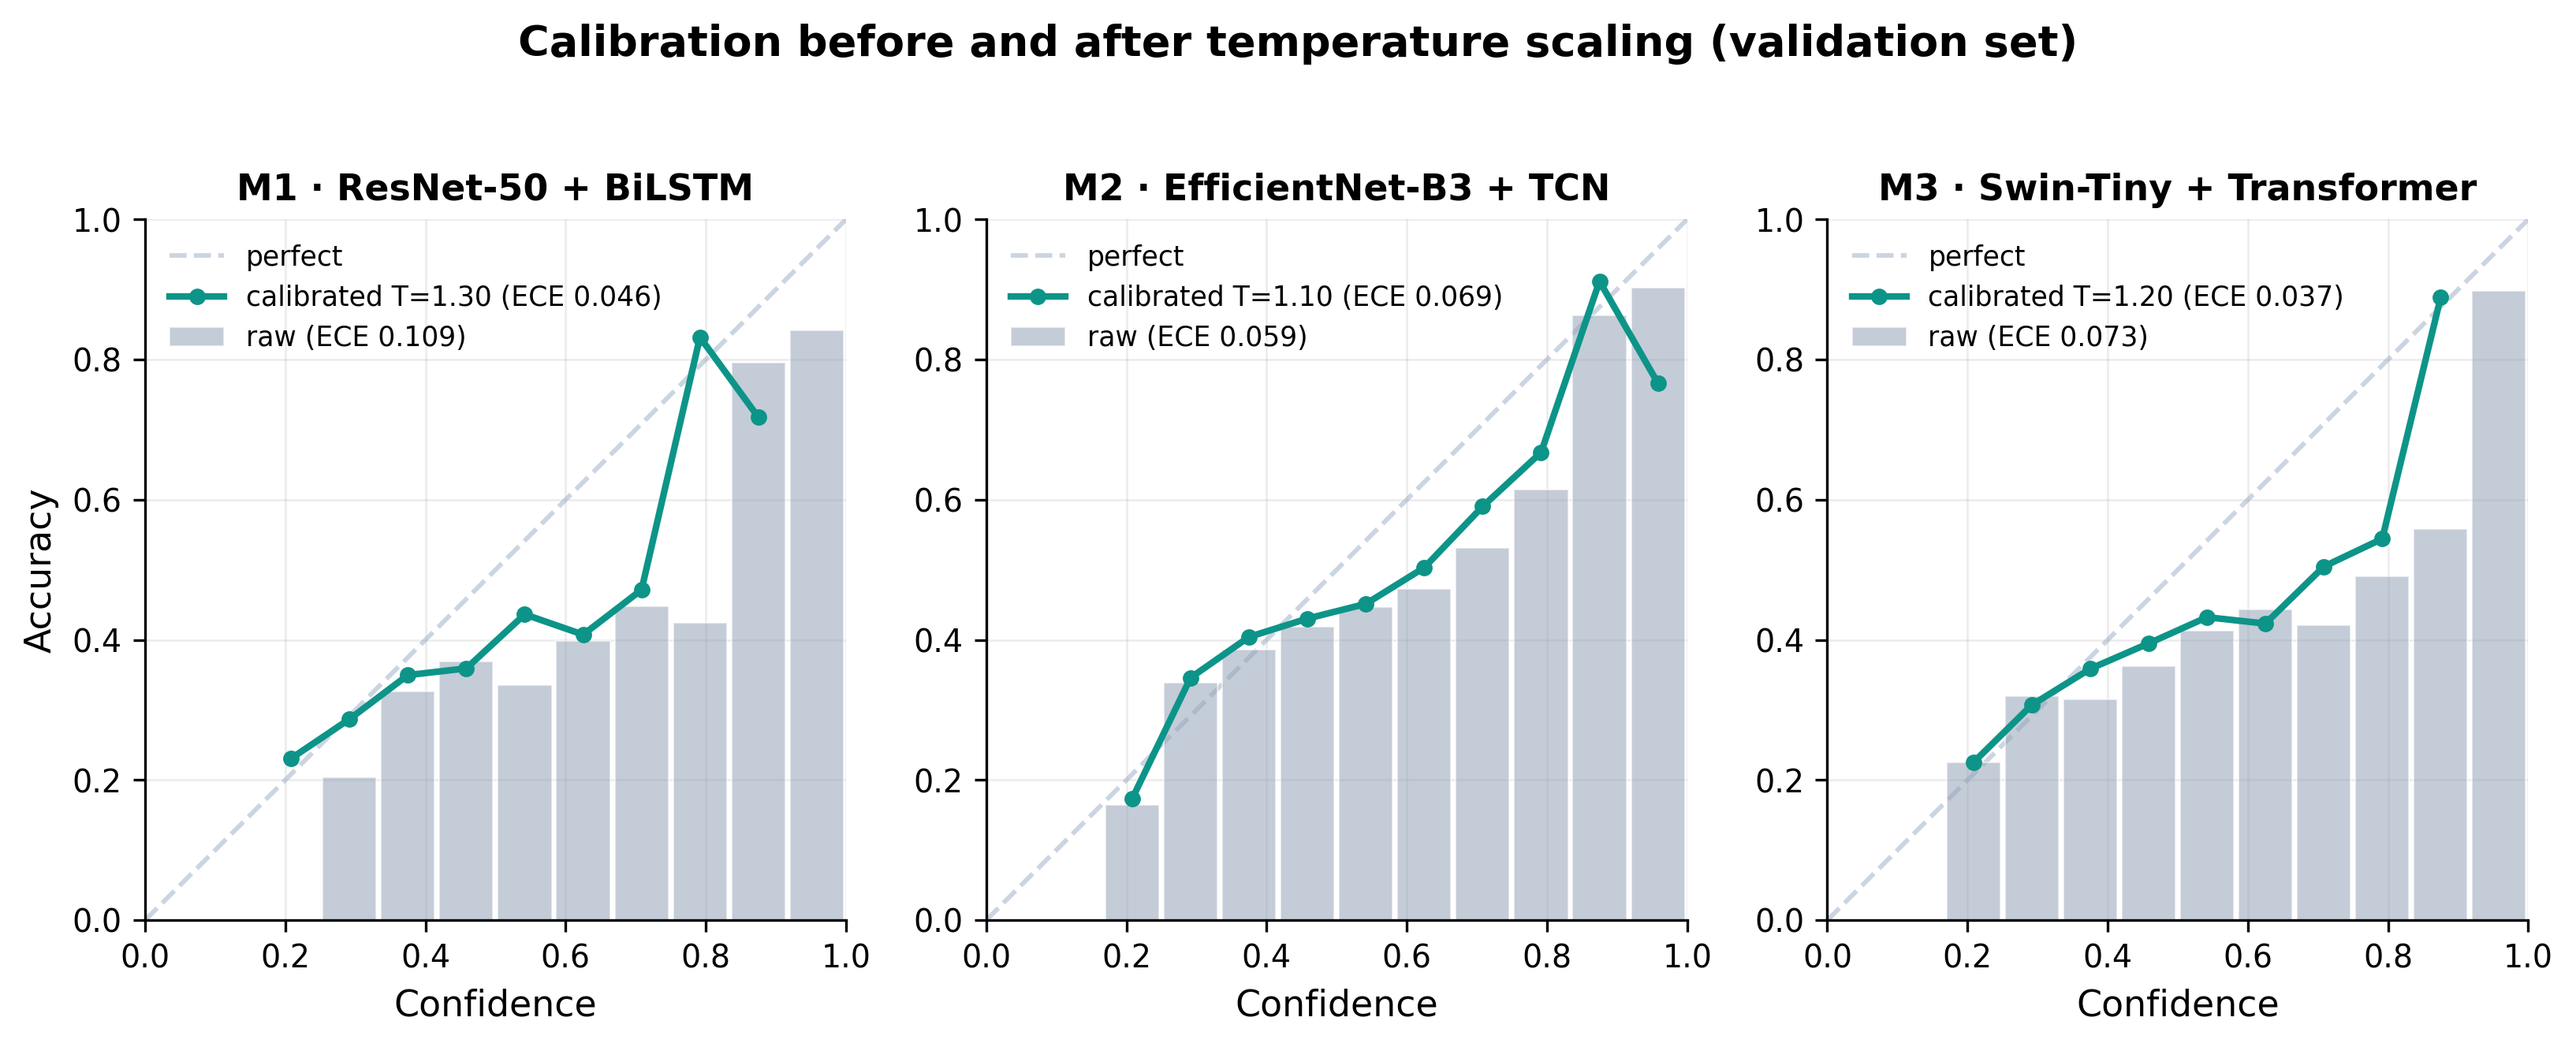
\includegraphics[width=\textwidth]{figures/reliability.png}
\caption{Biểu đồ độ tin cậy trên tập kiểm định. Cột xám là độ chính xác thô trong mỗi khoảng tin cậy; đường màu xanh là sau co giãn nhiệt độ; đường chéo nét đứt là hiệu chuẩn hoàn hảo. M1 dịch về phía đường chéo nhiều nhất.}
\label{fig:vn_reliability}
\end{figure}

\subsection{Đánh giá Bộ Giải mã}

Bảng~\ref{tab:vn_decoder} báo cáo độ chính xác và Macro-F1 trên tập kiểm tra cho mỗi bộ giải mã trên mỗi mô hình. Bộ giải mã được đề xuất (điểm số đã hiệu chuẩn cộng bảng chuyển pha) là bộ giải mã thời gian thực tốt nhất trên cả ba mô hình; bộ giải mã ngoại tuyến chỉ được nêu như một cận trên. Hình~\ref{fig:vn_benchmark} cho thấy cùng so sánh đó.

\begin{table}[H]
\centering
\caption{So sánh bộ giải mã (tập kiểm tra, độ chính xác / Macro-F1). Bộ giải mã ngoại tuyến $\dagger$ dùng các khung hình tương lai và chỉ là cận trên. Giá trị \emph{thời gian thực} tốt nhất in \textbf{đậm}.}
\label{tab:vn_decoder}
\begin{tabular}{lccc}
\toprule
\textbf{Bộ giải mã} & \textbf{M1 Acc / F1} & \textbf{M2 Acc / F1} & \textbf{M3 Acc / F1} \\
\midrule
Dự đoán thô              & 82,4 / 0,763 & 81,2 / 0,738 & 85,3 / 0,794 \\
Lọc trung vị-15          & 82,7 / 0,768 & 81,7 / 0,746 & 85,5 / 0,800 \\
Trình tự cố định + hc    & 82,5 / 0,777 & 82,4 / 0,767 & 86,0 / 0,802 \\
\textbf{Bộ giải mã đề xuất} & \textbf{83,0 / 0,771} & \textbf{82,9 / 0,764} & \textbf{86,0 / 0,806} \\
\midrule
Ngoại tuyến (toàn video) $\dagger$ & 91,8 / 0,859 & 91,8 / 0,849 & 90,1 / 0,832 \\
\bottomrule
\end{tabular}
\end{table}

\begin{figure}[H]
\centering
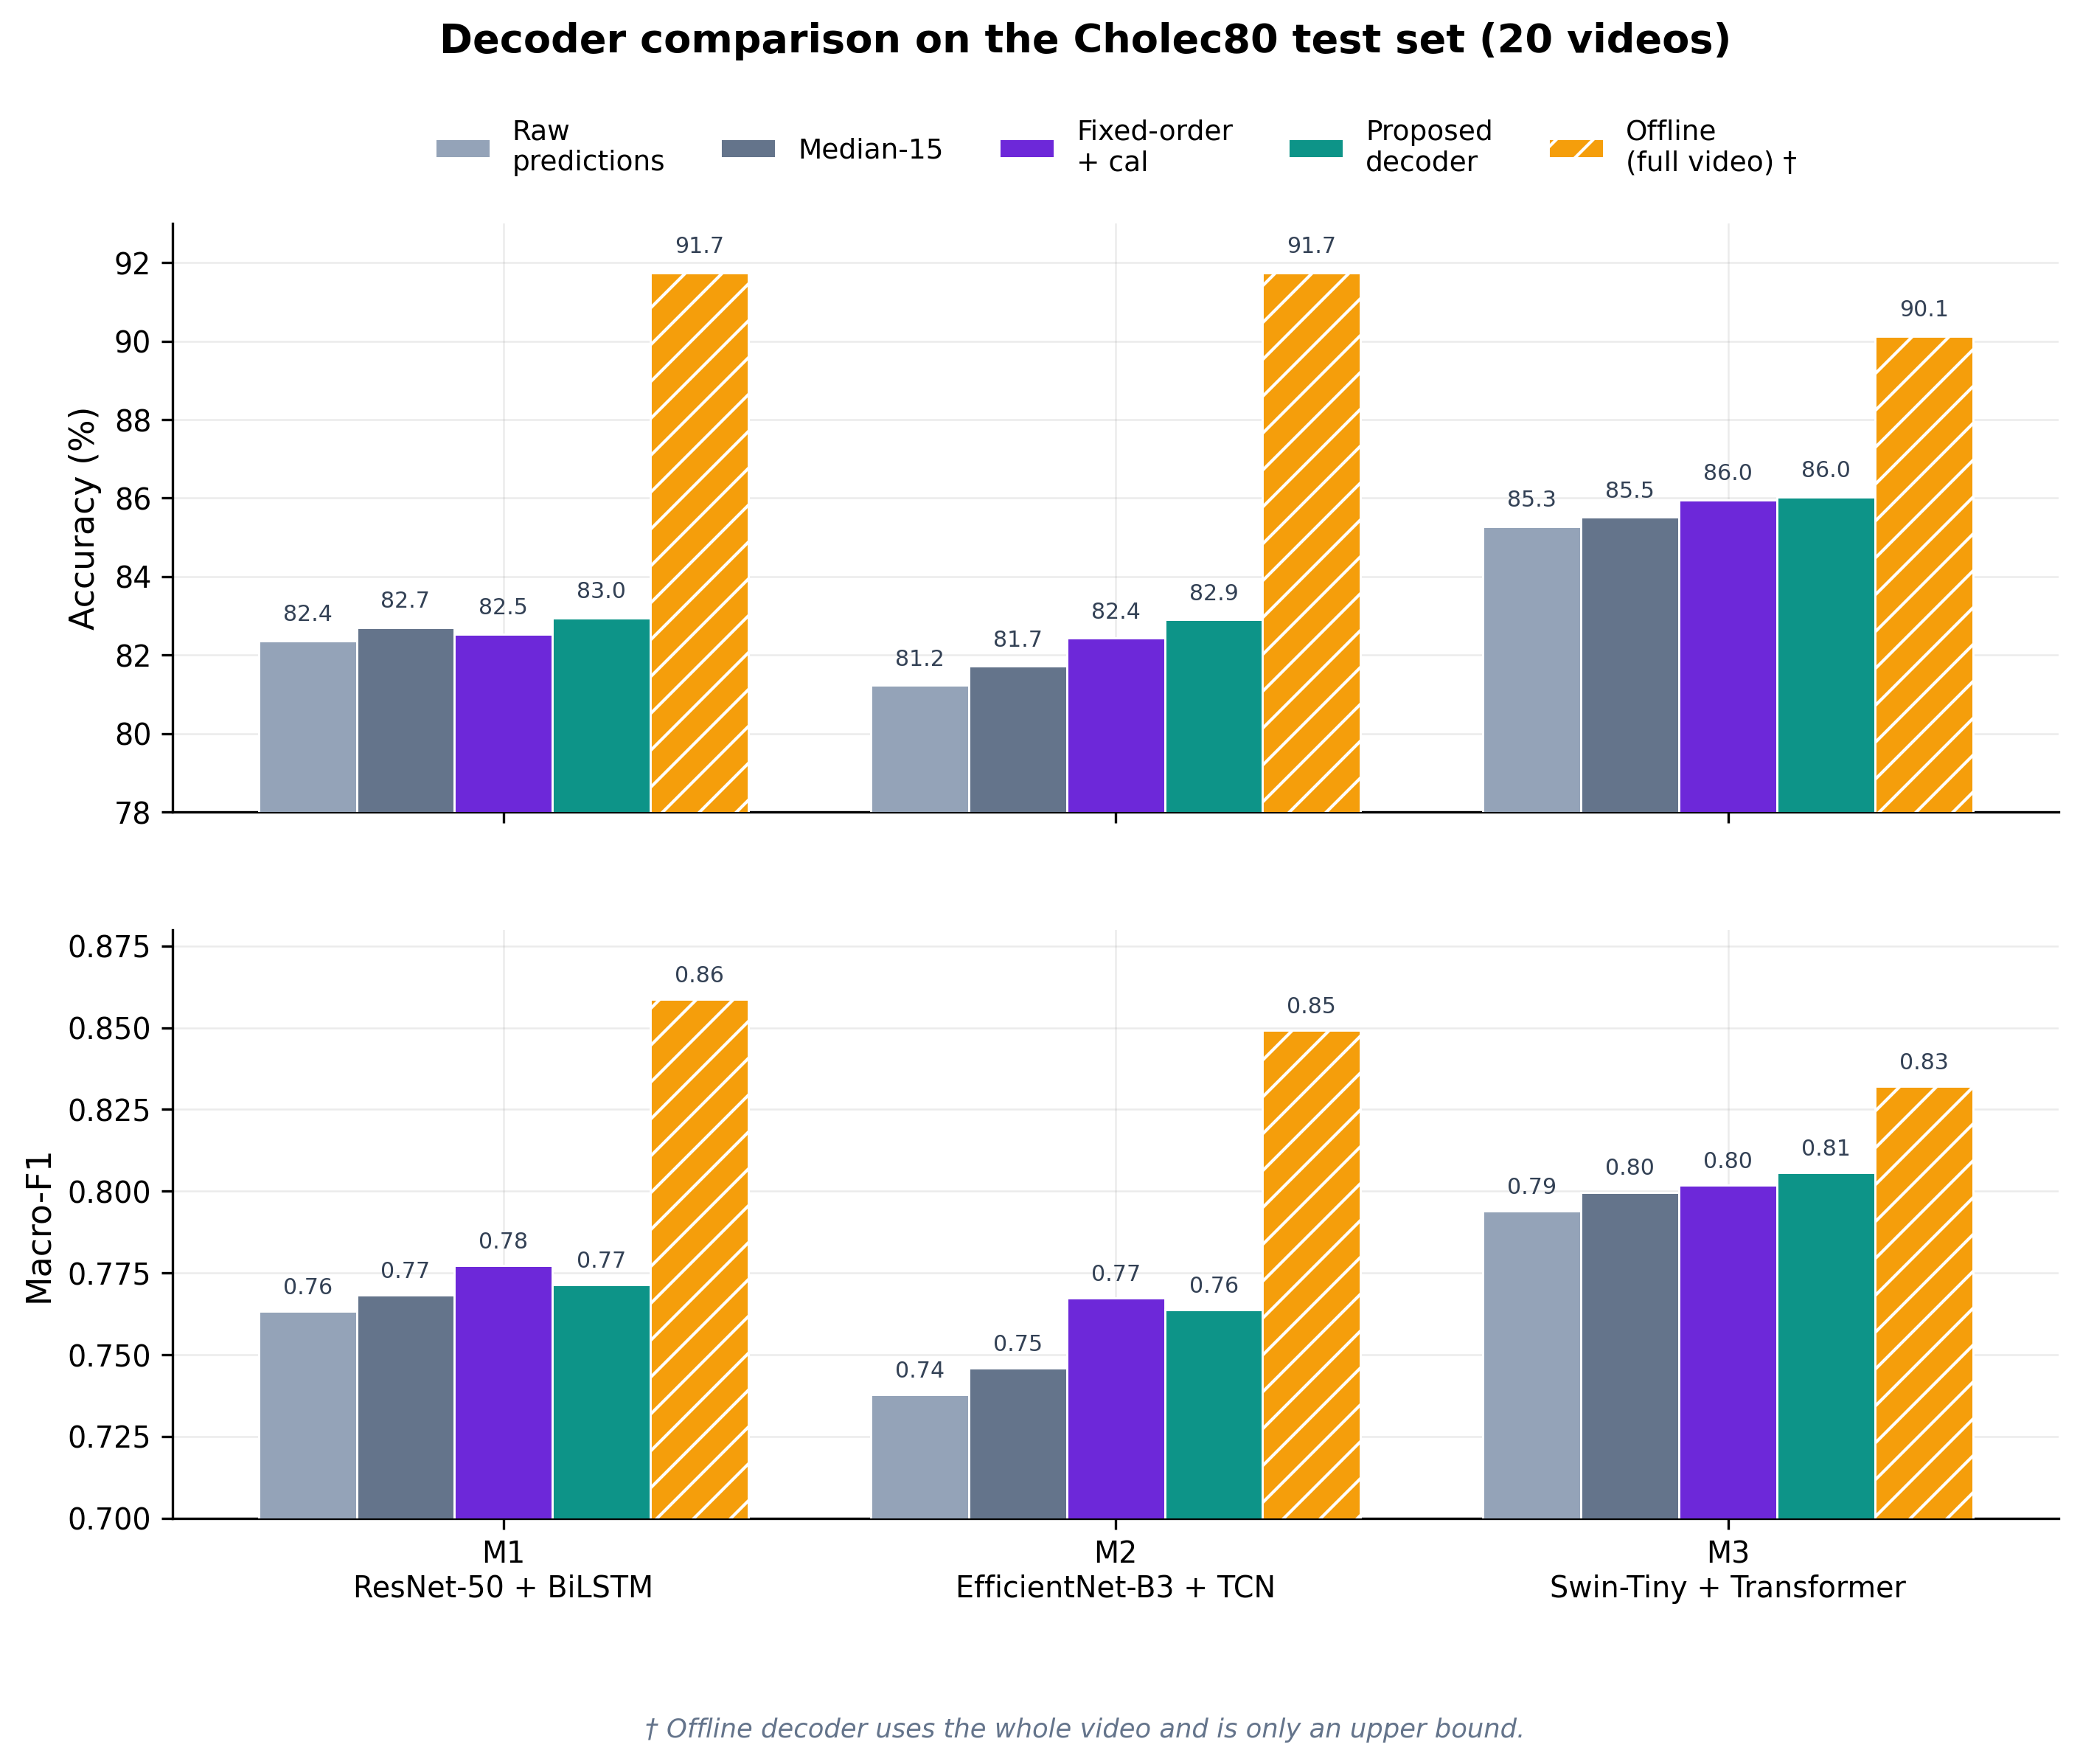
\includegraphics[width=\textwidth]{figures/benchmark.png}
\caption{So sánh bộ giải mã trên tập kiểm tra: độ chính xác và Macro-F1. Bộ giải mã đề xuất (màu xanh) là lựa chọn thời gian thực tốt nhất trên mọi mô hình; bộ giải mã ngoại tuyến (màu hổ phách, gạch chéo) dùng các khung hình tương lai và là cận trên.}
\label{fig:vn_benchmark}
\end{figure}

\subsection{Ý nghĩa Thống kê}

Vì các mức tăng trung bình trông nhỏ, một kiểm định ghép cặp theo từng video là quan trọng. Bảng~\ref{tab:vn_significance} báo cáo kiểm định Wilcoxon ghép cặp và hệ số Cohen $d$ trên hai mươi video kiểm tra, so sánh bộ giải mã đề xuất với dự đoán thô. Cả ba mô hình đều cho một cải thiện rõ ràng và nhất quán ($p < 0{,}001$, $d > 0{,}97$): mức tăng nhỏ về độ lớn nhưng đúng trên mọi video chứ không do một vài ngoại lệ. Bộ giải mã tốn 0,011--0,024~ms mỗi khung hình, thấp hơn nhiều so với 40~ms khả dụng giữa các khung hình trong video 25~fps. Hình~\ref{fig:vn_transition_significance} cho thấy bảng chuyển pha học được và các mức tăng theo từng video cạnh nhau.

\begin{table}[H]
\centering
\caption{Mức cải thiện theo từng video của bộ giải mã đề xuất so với dự đoán thô (20 video kiểm tra).}
\label{tab:vn_significance}
\begin{tabular}{lccc}
\toprule
\textbf{Mô hình} & \textbf{$\Delta$Acc (đpt)} & \textbf{Wilcoxon $p$} & \textbf{Cohen $d$} \\
\midrule
M1 --- ResNet-LSTM      & $+0{,}62$ & $<0{,}0001$ & 1,38 \\
M2 --- EffNet-TCN       & $+1{,}74$ & $0{,}0001$  & 1,25 \\
M3 --- Swin-Transformer & $+0{,}76$ & $0{,}0001$  & 0,98 \\
\bottomrule
\end{tabular}
\end{table}

\begin{figure}[H]
\centering
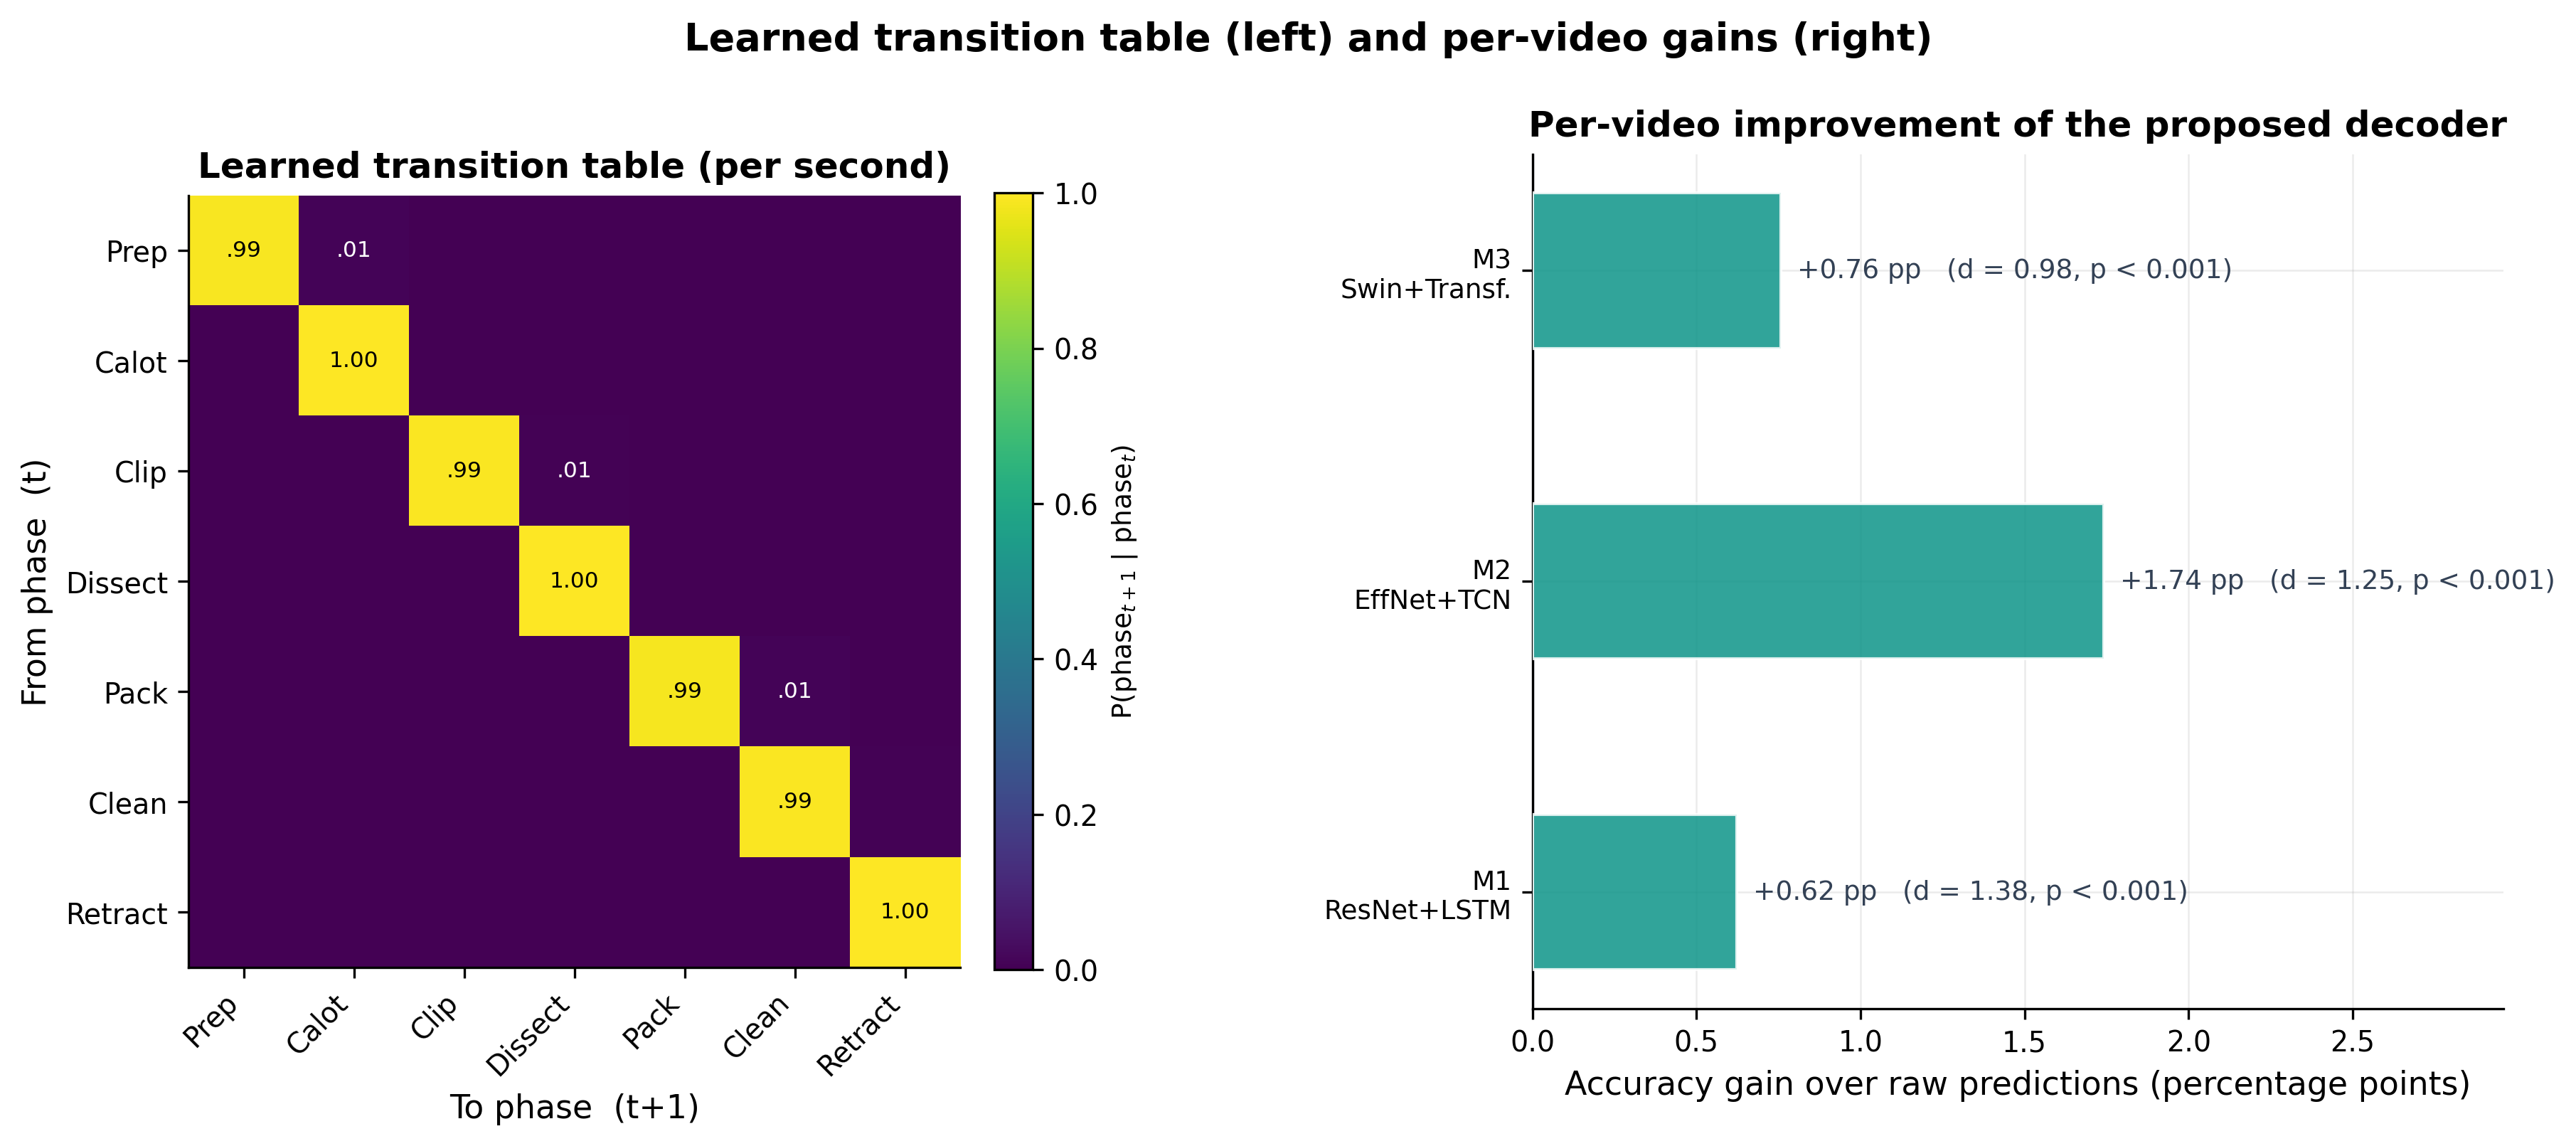
\includegraphics[width=\textwidth]{figures/transition_significance.png}
\caption{Trái: bảng chuyển pha mỗi giây học được, có đường chéo trội mạnh với phần trọng số còn lại nằm ở pha kế tiếp, khớp với trình tự pha cố định. Phải: mức tăng độ chính xác theo từng video của bộ giải mã đề xuất so với dự đoán thô, kèm hệ số Cohen $d$ và giá trị $p$ Wilcoxon.}
\label{fig:vn_transition_significance}
\end{figure}

\subsection{Ví dụ Minh họa}

Hình~\ref{fig:vn_timeline} cho thấy dòng thời gian pha dự đoán cho một video kiểm tra. Các dự đoán thô đổi qua đổi lại, nhất là ở đoạn đầu; bộ giải mã đề xuất loại bỏ phần lớn các lần đổi này và bám theo nhãn thật sát hơn nhiều.

\begin{figure}[H]
\centering
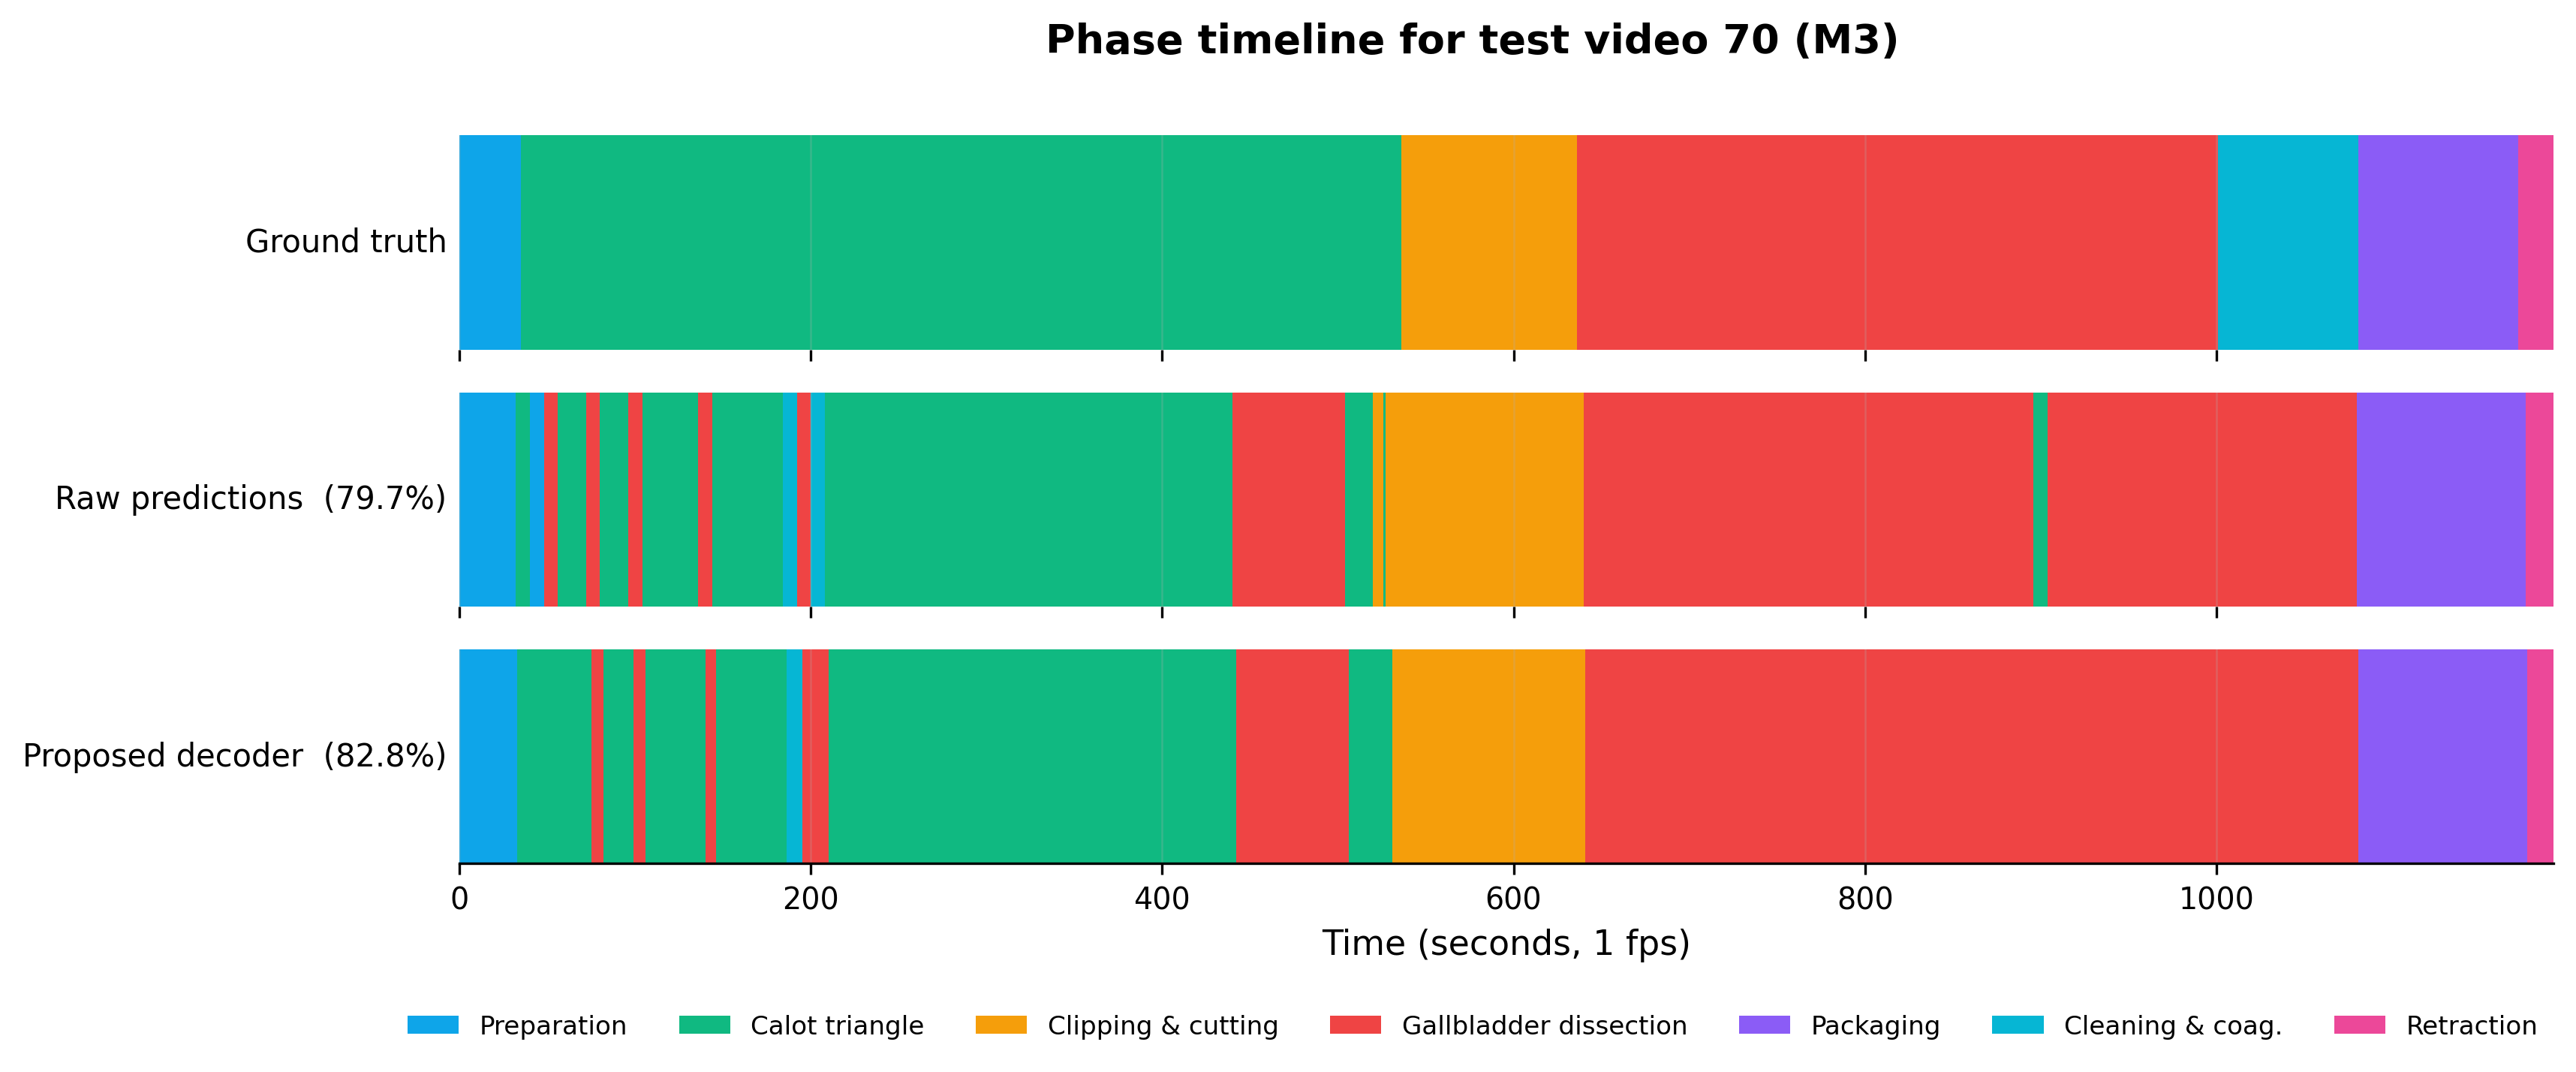
\includegraphics[width=\textwidth]{figures/timeline.png}
\caption{Dòng thời gian pha cho một video kiểm tra (M3). Các dự đoán thô (giữa) đổi nhãn thường xuyên; bộ giải mã đề xuất (dưới) mượt hơn hẳn và bám sát nhãn thật (trên).}
\label{fig:vn_timeline}
\end{figure}

\section{Lỗi Gần Điểm Chuyển pha so với Bên trong Pha}
\label{sec:vn_boundary}

Trên Cholec80, sự bất đồng về nhãn tập trung ở các điểm chuyển pha, nơi ngay cả người gán nhãn cũng khác nhau về thời điểm chính xác của chuyển tiếp. Để thấy mỗi bộ giải mã giúp ích ở đâu, các khung hình kiểm tra được chia thành nhóm \textbf{gần một điểm chuyển pha} (trong khoảng $\pm5$~giây quanh một chuyển tiếp thật) và nhóm \textbf{bên trong một pha} (mọi chỗ còn lại). Bảng~\ref{tab:vn_boundary} báo cáo cách chia này cho M3, và Hình~\ref{fig:vn_boundary} minh họa nó.

\begin{table}[H]
\centering
\caption{Độ chính xác gần điểm chuyển pha so với bên trong pha, cho M3. Bộ giải mã ngoại tuyến $\dagger$ dùng các khung hình tương lai. Giá trị \emph{thời gian thực} tốt nhất in \textbf{đậm}.}
\label{tab:vn_boundary}
\begin{tabular}{lcc}
\toprule
\textbf{Bộ giải mã} & \textbf{Gần chuyển pha} & \textbf{Bên trong pha} \\
\midrule
Dự đoán thô              & 60,7\% & 86,1\% \\
Lọc trung vị-15          & 61,1\% & 86,3\% \\
\textbf{Bộ giải mã đề xuất} & \textbf{63,2\%} & 86,8\% \\
\midrule
Ngoại tuyến (toàn video) $\dagger$ & 62,8\% & 91,0\% \\
\bottomrule
\end{tabular}
\end{table}

\begin{figure}[H]
\centering
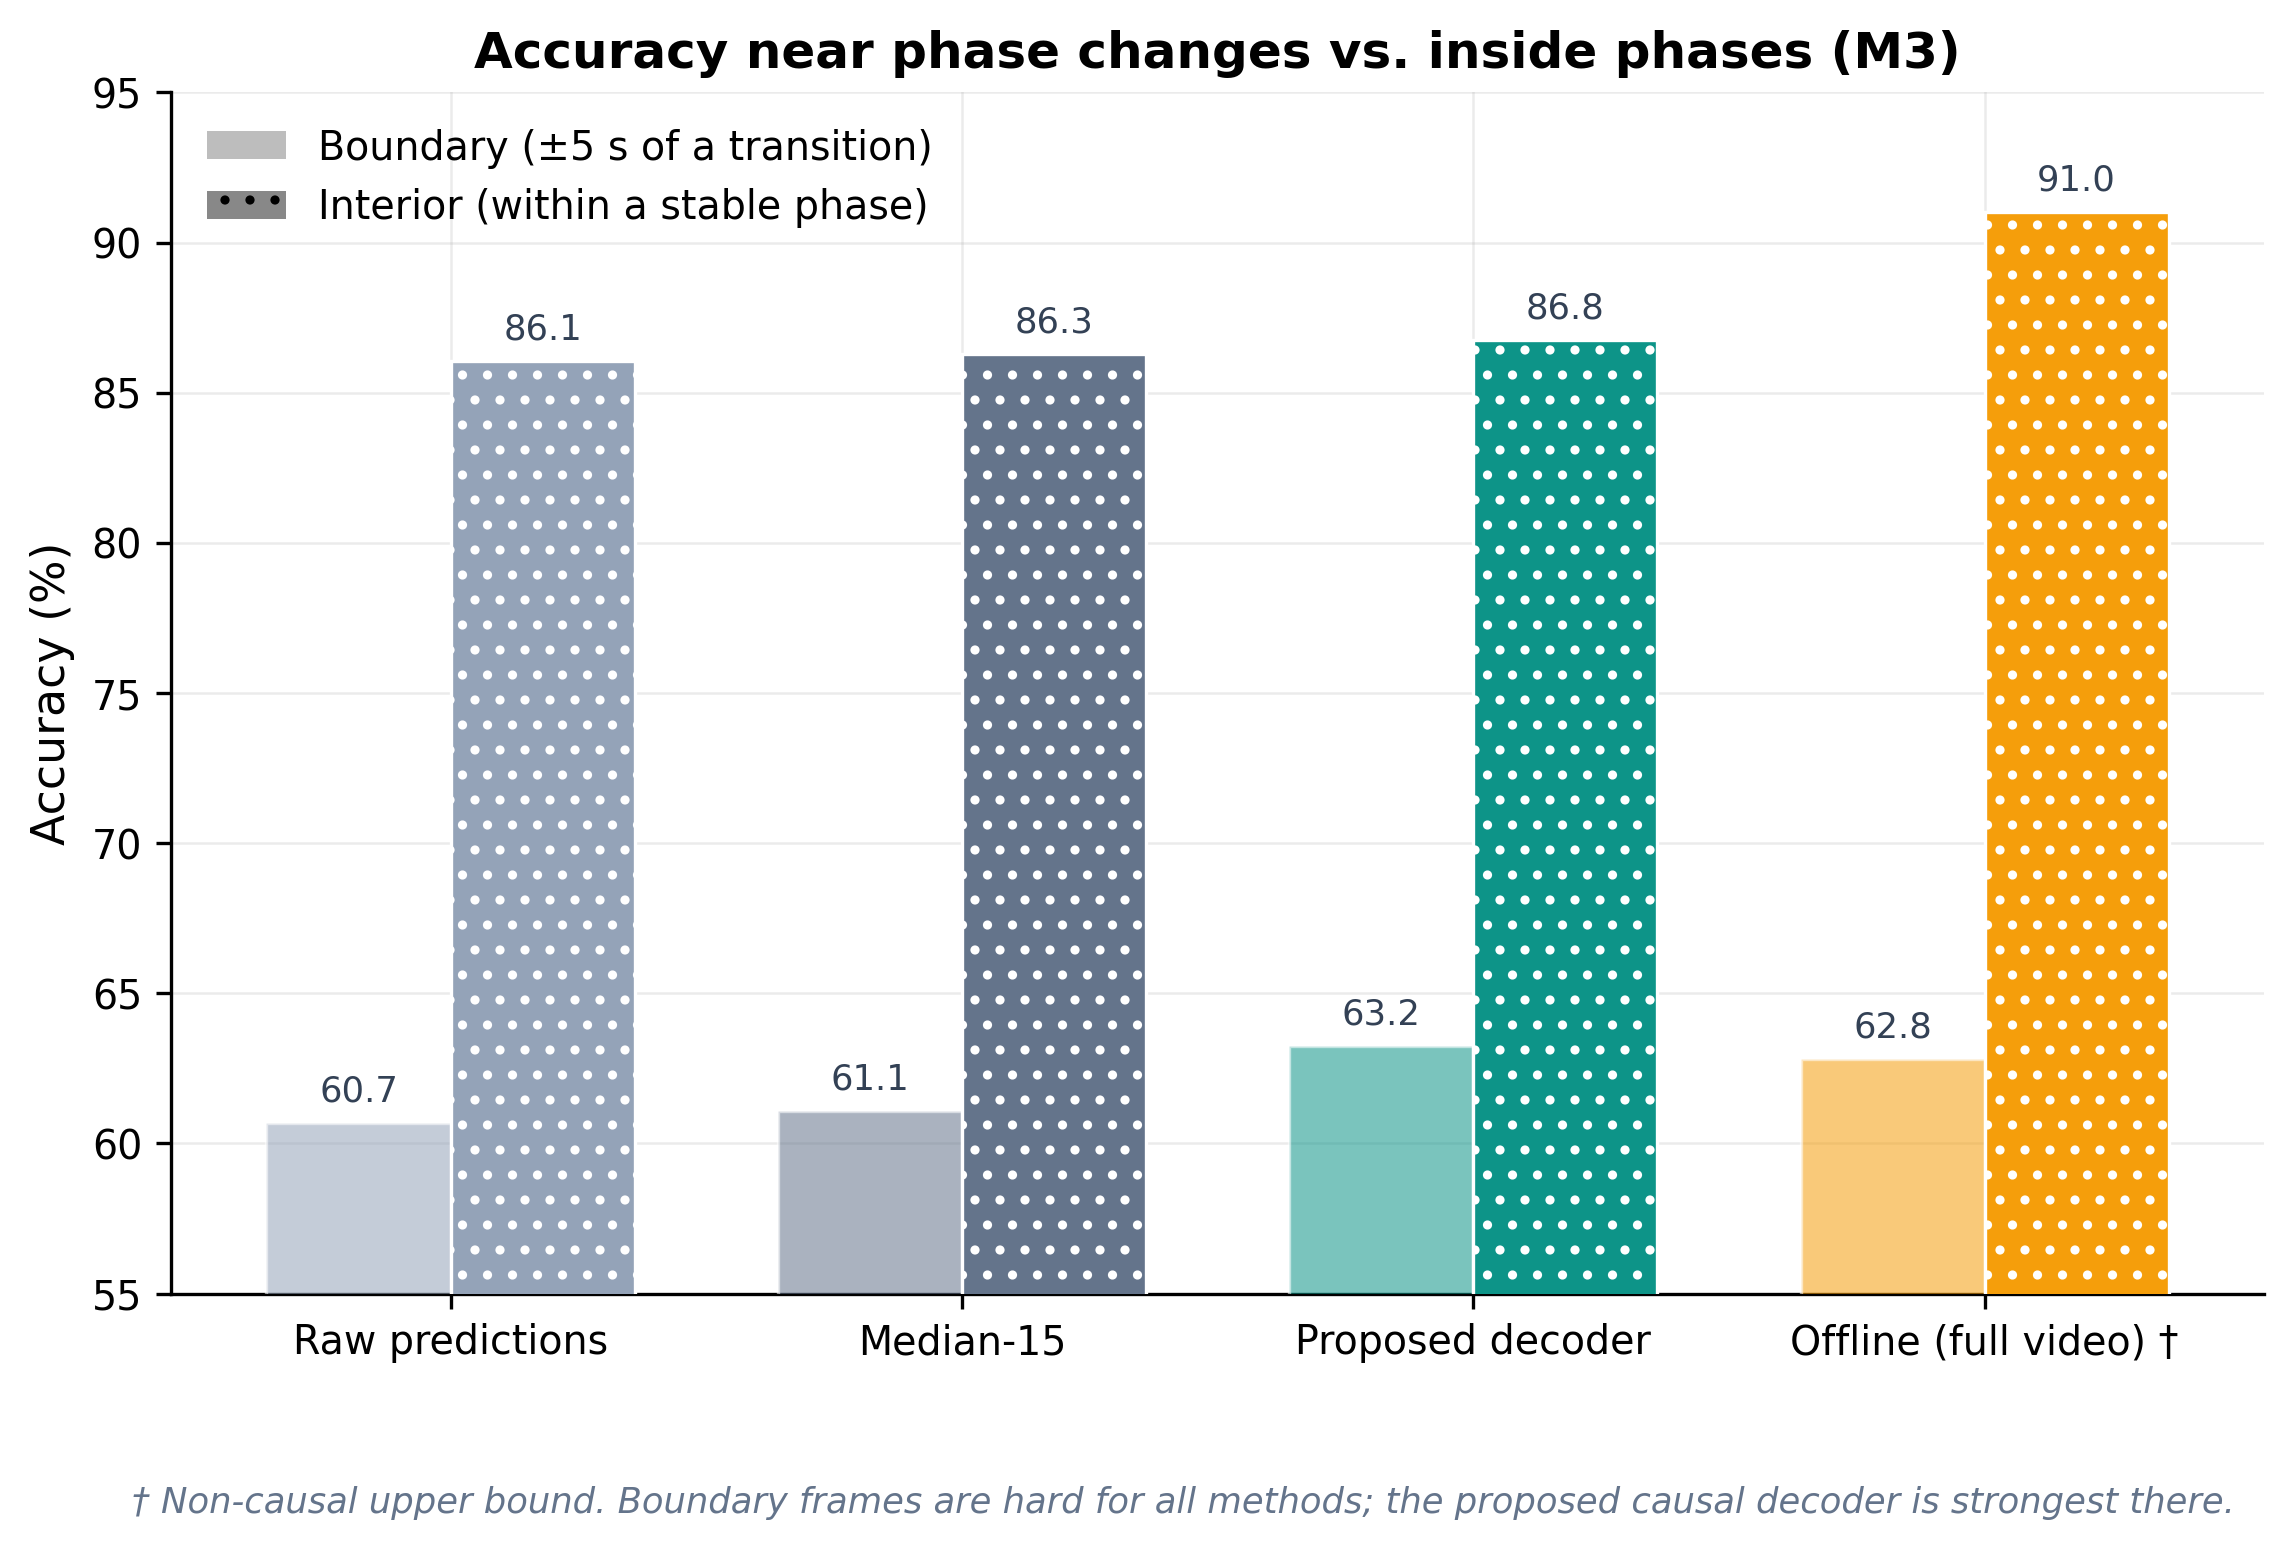
\includegraphics[width=\figwidth]{figures/boundary.png}
\caption{Độ chính xác gần điểm chuyển pha so với bên trong pha, cho M3. Các khung hình gần chuyển pha (cột đặc) khó với mọi phương pháp; bộ giải mã đề xuất tốt nhất ở đó, thậm chí hơi cao hơn cả cận trên ngoại tuyến. Bên trong pha (cột gạch chéo) là nơi ưu thế của bộ giải mã ngoại tuyến đến từ.}
\label{fig:vn_boundary}
\end{figure}

Hai điểm nổi bật. Thứ nhất, bộ giải mã đề xuất \textbf{tốt nhất ở gần điểm chuyển pha} (63,2\%), thậm chí trên cả cận trên ngoại tuyến (62,8\%): quy tắc cứng của bộ giải mã ngoại tuyến rằng pha không thể đi lùi đôi khi làm trễ một chuyển tiếp, trong khi bảng học được mềm dẻo hơn nên bám theo thời điểm chuyển nhãn linh hoạt hơn. Thứ hai, toàn bộ khoảng cách 4,2 điểm giữa bộ giải mã ngoại tuyến và bộ giải mã thời gian thực tốt nhất nằm \emph{bên trong} các pha ($86{,}8 \to 91{,}0$), không phải ở các điểm chuyển. Ưu thế của bộ giải mã ngoại tuyến là sửa các lỗi thoáng qua bên trong các pha dài ổn định bằng cách nhìn các khung hình tương lai --- điều mà một bộ giải mã thời gian thực không thể làm. Theo hiểu biết của chúng tôi, cách chia này chưa từng được đo trên Cholec80, và nó chỉ ra một bước tiếp theo rõ ràng: cho phép bộ giải mã nhìn trước vài giây sẽ thu hẹp phần lớn khoảng cách mà vẫn dùng được gần như thời gian thực.
